\documentclass[times, utf8, seminar]{fit}

%\batchmode
%\usepackage{booktabs}
\usepackage{listings}
\usepackage{longtable}
\usepackage{xcolor}
\usepackage{float}
\usepackage{enumitem}
\usepackage{hyperref}

\begin{document}

\title{Poslovna inteligencija bazirana na "open source" software-u}

\author{Ernad Husremović}
\brindex{DL 2792}
\verzija {1.9.8}

\mentor{prof.dr Vanja Bevanda}

\maketitle

\tableofcontents

\chapter{Uvod}

\section{Poslovna inteligencija (BI)}

Poslovna inteligencija (nadalje BI\footnote{BI Business intelligence}) se primarno odnosi na računarski bazirane tehnike identificiranja, ekstrakcije i analize poslovnih podataka.  BI tehnologije obezbjeđuju pregled ranijih i tekućih poslovnih operacije, kao i predviđanje budućih trendova u poslovanju\footnote{prediktivna analiza} \cite{web:wikipedia:bi}.

Standardne funkcije BI-a su:

\begin{enumerate}
  \item izvještavanje (reporting)
  \item analitičko procesiranje (analitycal processing)
  \item rudaranje podataka (data mining)
  \item prediktivne analize (predictive analytics)
\end{enumerate}

Sve ove funkcije pomažu poslovnom odlučivanju i planiranju - kako strateškom\footnote{Odlučivanje `top' managera} tako i operativnom planiranju\footnote{`department' manageri}.

\subsection{Operativni podaci, skladišta podataka}
\label{operativni_podaci}

BI kao izvor podataka koristi skladišta podataka.

Skladišta podataka treba razlikovati od operativnih podataka. Operativni podaci - podaci o tekućem poslovanju nalaze se unutar poslovnih aplikacija (ERP)\footnote{ERP - Enterprise Resource Planning software, software za podršku tekućem poslovanju}.

ERP sistemi pohranjuju poslovne transakcije (poslovne dokumente) u realnom vremenu.

ERP sistemi sadrže sisteme izvještavanje\footnote{traditional reporting} koji su primarno usmjereni na davanje podataka o tekućem poslovanju\footnote{period tekuće poslovne godine}.

Operativni podaci su glavni izvor za gradnju skladišta podataka. Međutim, skladišta podataka se najčešće grade iz heterogenih izvora.

Iako slični po načinu konstrukcije, u BI terminologije se pravi distinkcija  između `data mart' i `data warehouse' skladišta podataka\footnote{U domaćoj literaturi se najčešće za oba pojma koristi termin `skladište podataka'}:  

\begin{description}
  \item [Data mart (DMart)] sadrži informacije o jednom dijelu organizacije (npr. prodaja, ljudski resursi),
  \item [Data warehouse (DW)] sadrži informacije iz više područja - obrađuje organizaciju globalno.
\end{description}
 
DW je stoga usmjeren na podršku 'top' menadžmenta, dok 'datamart' obezbjeđuje informacije za upravljanje i operativno planiranje pojedinih dijelova organizacije \cite[str.~391]{pentaho32}.

\section{Poslovni motivi za realizaciju sistema BI-a}

Analiza poslovnih podataka radi kvalitetnog poslovnom odlučivanja je postojala i prije informatičke podrške poslovanju.

Slijedeća poslovna pitanja su postavljana i prije informatičke ere:

\begin{itemize}
  \item Kako se kretala prodaja određene grupe artikala u predhodnom periodu ?
  \item Koja grupa artikala se najviše zadržava na lageru ?
  \item Kakva je struktura prodaje po regijama ?
  \item Unutar koje grupacije artikala / proizvoda je najbolja marža ?
\end{itemize} 


Sva ova pitanja praktično vrše analizu efekata poslovanja usljed različitih uticaja (multidimenzionalna analiza).

Iz svih gornjih pitanja mogu se uočiti dva tipa informacija:

\begin{itemize}
   \item mjere - poslovni indikatori (prodaja, vrijednost zalihe, visina marže)
   \item dimenzije - atributi poslovanja (geografske dimenzije - grad, region, vemenske dimenzije, grupe artikala, rang cijena ...)
\end{itemize}

Ovo je bilo polazište za konstrukciju multidimenzionalnih skladišta podataka (OLAP cube).
 
\subsection{OLAP kocka}

OLAP kocka  (OLAP cube\footnote{OLAP - online analytical processing}) je set podatka organizovanih na taj način da omogućavaju \emph{nedeterminirane} upite nad agregiranim podacima, odnosno online analitičko procesiranje podataka \cite{web:wikipedia:olap_cube}.

Ovakva organizacija podataka omogućava OLAP klijentima pregled podataka u različitim varijantama.

Ono što RDBMS\footnote{RDBMS relational database management system} predstavlja za ERP sistem, OLAP kocka predstavlja za BI sistem.

Analogija postoji i u dijelu pretrage podataka:

\begin{itemize}
 \item RDBMS <-> SQL structured query language
 \item OLAP cube <-> MDX - multidimensional query language
\end{itemize}

Današnje implementecije OLAP kocki:

\begin{itemize}
  \item ROLAP - podaci smješteni u relacijske baze podataka
  \item MOLAP - podaci su u proprietary formatu prilagođenom procesiranju multidimenzionalnih struktura podataka
\end{itemize}

Pored gornjih postoje i hibridne implementacije OLAP kocki koje kombinuju obje tehnologije.

\subsection{Alati za integraciju podataka (DI)}

DI\footnote{DI - data integration} alati mogućavaju vezu BI sistema sa "vanjskim" svijetom (vidi \ref{operativni_podaci} operativni podaci)

Glavni dio DI `toolset'-a su je ETL softver\footnote{ETL - Extract/Transform/Load}. 

ETL softver obavlja sljedeće funkcije:

\begin{enumerate}
  \item \emph{Extract:}  uzimanje podataka iz vanjskih izvora
  \item \emph{Transform:} izvrši transformaciju podataka u format koji je pogodan za pohranu u DW odnosno DMart (vidi \ref{operativni_podaci})
  \item \emph{Load:} konačno snimi podatke `prečišćene' u predhodnom koraku podatke u DW/DMart
\end{enumerate}
 
\subsection{Rudarenje podataka}

Pojam rudaranje podataka se može definisati kao pronalaženje zakonitosti među podacima. 

Jedna od definicija rudaranje glasi: rudarenje podataka je sistematičan, interaktivan i iterativan proces izvođenja i prikazivanja korisnika, implicitnog i inovativnog \emph{znanja} iz podataka \cite[str.~40]{mag_mrsic}.

Unutar ovog rada nećemo se baviti ovim dijelom BI-a.

Open source software koji pokriva ove oblasti:
 
\begin{itemize}
  \item Data mining `Weka' projekat: \cite{web:weka}, \cite{web:pentaho_weka}
  \item `R' statistički paket \cite{web:r}
\end{itemize}

Treba uočiti da je `Weka' jedan od podprojekata `Pentaho BI suite'-a (vidi \ref{sect:pentaho}).

\chapter{`Open source' BI software}

`Open source' sofware pokriva komletan opseg alata

\section{Pentaho BI}

Pentaho BI obuhvata praktično funkcije BI-a \cite[str.~7]{pentaho32}:

\begin{enumerate}
 \item multidimenzionalna analiza
 \item reporting
 \item `dashboards' - prikaz glavnih poslovnih indikatora
\end{enumerate}

\begin{figure}[H]
\centering
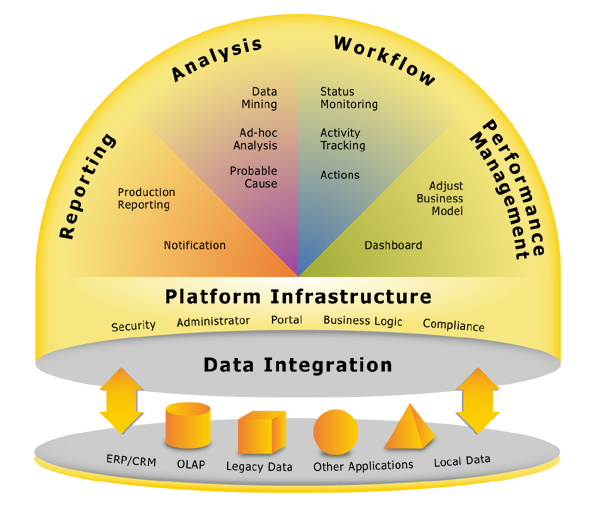
\includegraphics[width=12cm]{img/pentaho_arhitektura_eric.png}
\caption{Pentaho arhitektura (\cite{web:eric})}
\end{figure}

\section{Pentaho komponente}
\label{sect:pentaho}

\subsection{Mondrian OLAP}

Pentaho implementacija OLAP kocke naziva se `Mondrian'. Mondrian je kocka ROLAP tipa.

Bitno je naglasiti da je `Mondrian'  XMLA kompatibilan provajder\footnote{XML za Analizu (XMLA) je industrijski standard za pristup podacima u analitičkim sistemima kao što su OLAP i `data mining'. Baziran je na drugim industrijskim standardima kao što su XML, SOAP i HTML \cite{web:wikipedia:xmla}.}


\subsection{Mondrian OLAP schema} 

Kao ROLAP implementacija, podaci se nalaze u relacijskog bazi podataka\footnote{Podržane su sve JDBC podržane relacijske baze: PostgreSQL, MySQL, MSSQL, Oracle}

Kod konstrukcije sheme koriste se sljedeći pojmovi:

\begin{itemize}
  \item `dimension table' - tabela u kojoj su pohranjene dimenzije
  \item SCD slow changing dimension
  \item SCD Type I - čuva se samo jedna vrijednost dimenzije
  \item SCD Type II - čuva se istorija vrijednosti dimenzije kroz vremenski period \footnote{npr. cijena artikla se mijenja tokom vremena, SCD type II dimenzija za svaku novu cijenu pravi novi zapis u dimension tabeli}
  \item `facts table' - tabela u kojoj su mjere - poslovni indikatori koje analiziramo
  \item `business key' (bk) - ključ koji koriste aplikacije za rukovanje operativnim podacima (ERP software)
  \item `surogat key' (id) - ključ u bazi podataka koji koristi OLAP storage
  \item `snowflake' schema - šema u kojoj su dimenzije u sopstvenim tabelama, dimenzije su visokog stepena normalizacije podataka\footnote{normalizacija podataka u relacijskog bazi podataka} \cite{web:pentaho:mondrian_schema}
  \item Type II
\end{itemize}

Pogledajmo jednu gotovu mondrian schemu (vidi \ref{chap:case_study} dobijenu u narednom \emph{case study}-ju):

\begin{figure}[h]
\centering
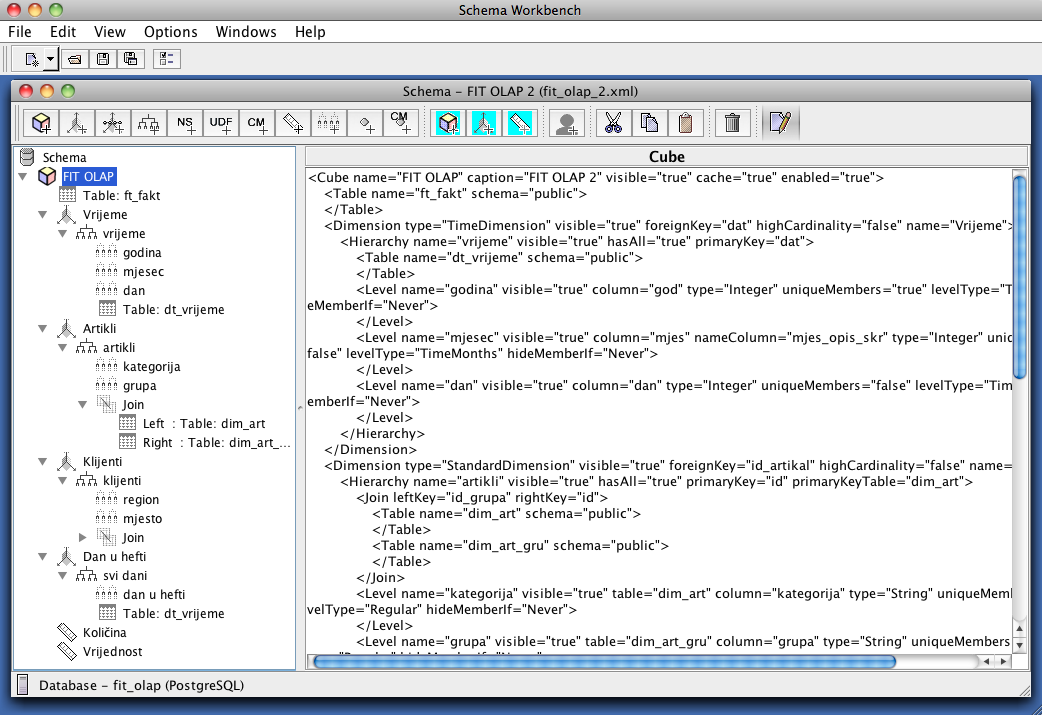
\includegraphics[width=15cm]{img/fit_olap_mondrian_schema}
\caption{Mondrian schema OLAP 2 cube}
\end{figure}


\section{Pentaho ETL dizajner `Spoon'}

`Spoon' GUI aplikacija u kome se vrši definicija i testiranje ETL transformacija i `job'-ova.

Kod ETL operacija bitno je poznavati sljedeće pojmove:

\begin{itemize}
  \item 'cleansing` - "čišćenje" podataka - ispravka (ili izbacivanje) netačnih podataka
\end{itemize}

\subsection{OALP Analyzer}

Pentaho sadrži dva `OLAP analyzer'\footnote{OLAP cube consumer} rješenja:

\begin{itemize}
  \item JPilot - starije rješenje, napušta se njegov razvoj\footnote{označeno od Pentaho razvojnog tima kao `depreated'}
  \item novi `OLAP Analyzer' koji se nalazi samo u `Enterprise' (plaćenoj verziji)\footnote{znači ova komponenta je `closed source' sofware tako da se u ovom radu neće dalje razmatrati.}
\end{itemize}

Kao `OLAP Analysis' sofver korišten je Saiku.

Saiku je modularni open-soruce analitički sotver koji nudi jednostavnu OLAP analizu podataka \cite{web:saiku}

OLAP analitički softver barata sa sljedećim pojmovima:

\begin{itemize}
  \item redovi - sadrži jednu ili više mjera ili dimenzija koje se prikazuju u redovima kod prikaza podataka
  \item kolona - sadrži jednu ili više mjera ili dimenzija koji se prikazuju u kolonama prikaza podatka
  \item filteri - ograničenje podataka po određenim vrijednostima dimenzija
\end{itemize}

\chapter{OLAP Case study}
\label{chap:case_study}

U ovom `case study'-ju ćemo izvršiti formiranje OLAP kocke za operativne podatke ERP aplikacije `F18 knowhow'. U DMart ćemo staviti podatatke za sve aktivne poslovne godine firme "bring.out" (1996-2011). 

\section{F18 knowhow ERP}

\begin{figure}[H]
\centering
\includegraphics[width=15cm]{img/F18_erp.png}
\caption{ERP aplikacija, F18 klijent}
\end{figure}

\section{Poslovni cilj analize}

Cilj je analizrati prodaju firme po godinama pri čemu nas interesuje struktura klijenata po gradovina i regionima, te prodaja artikala po određenim kategorijama i grupama.

Glavni Operativni podaci nalaze se u ERP aplikaciji, u PostreSLQ relacijskoj bazi. 

Dio potrebnih dimenzija (regioni, kategorije i grupe artikala) nisu implementirani unutar operativnih podataka, tako da analitičar mora unutar ETL procesa ove informacije dodati. 

Podaci svake poslovne godine nalaze se u posebnoj bazi podataka.

Operativni podaci `F18 knowhow' smješteni su u sljedeći relacijski model:

\begin{figure}[H]
\centering
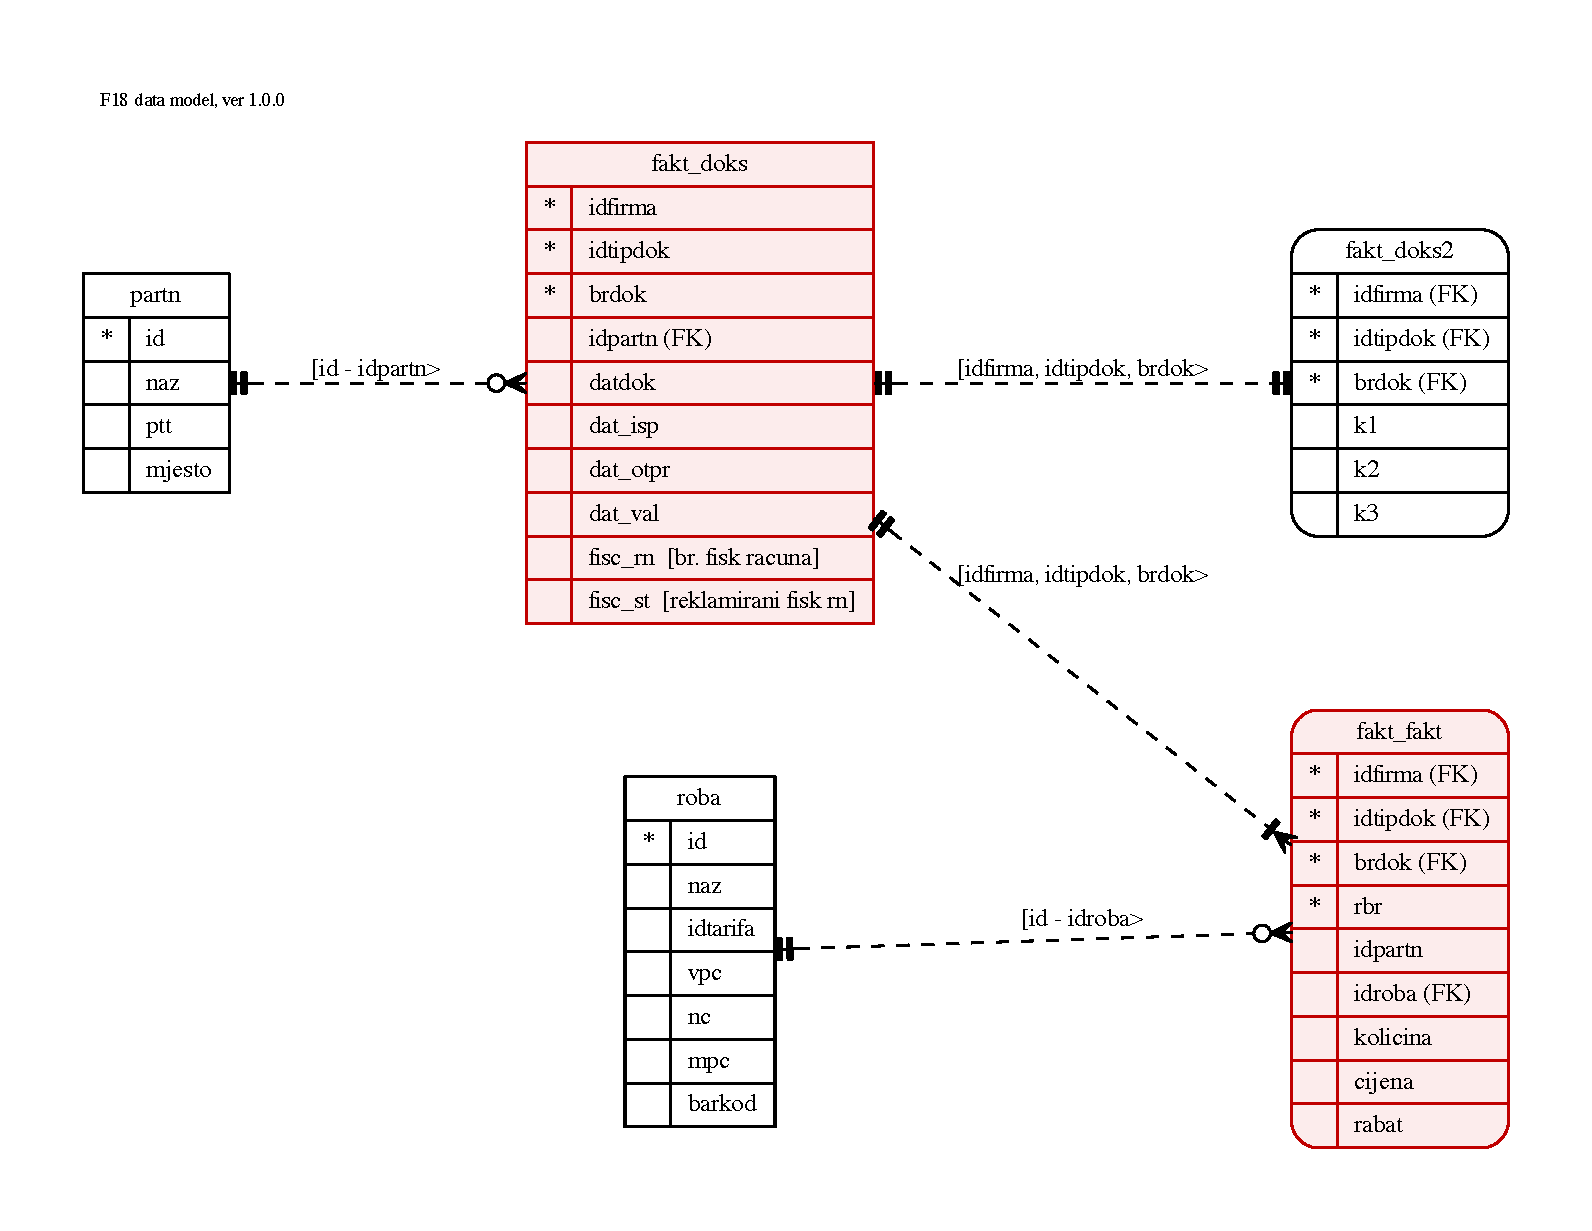
\includegraphics[width=15cm]{img/F18_db.pdf}
\caption{F18 transakcijski db model (relevantni dio)}
\end{figure}


F18 `cleansing' podaci  (Dodatak \ref{chap:izvorni_kod}, olap\_cleansing `spreadsheet' dokument)

Klasificiranje izvornih podataka - šifrarnik artikala

\begin{figure}[H]
\centering
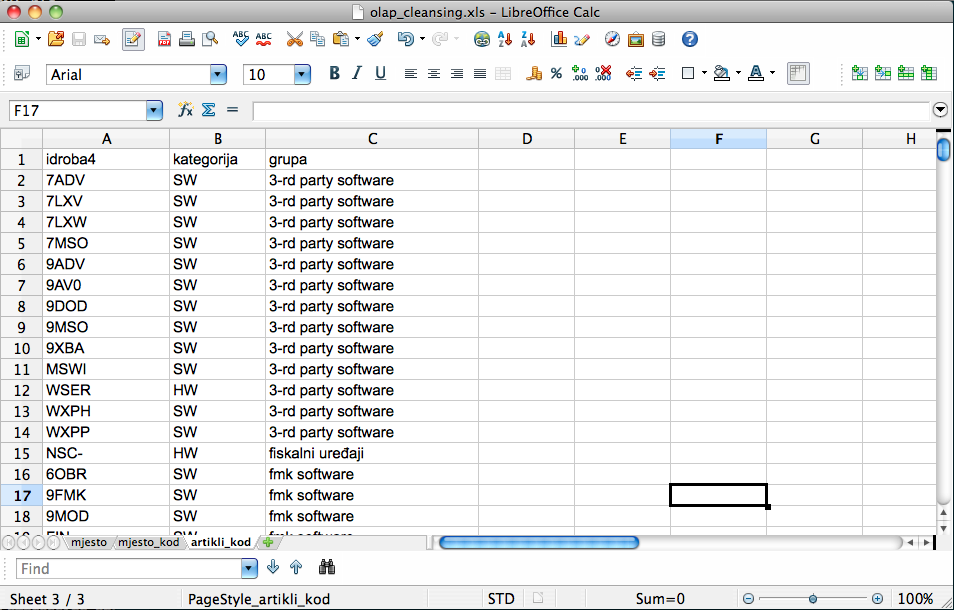
\includegraphics[width=15cm]{img/clean_artikli.png}
\caption{F18 klasificiranje - šifarski sistem artikala}
\end{figure}



\begin{figure}[H]
\centering
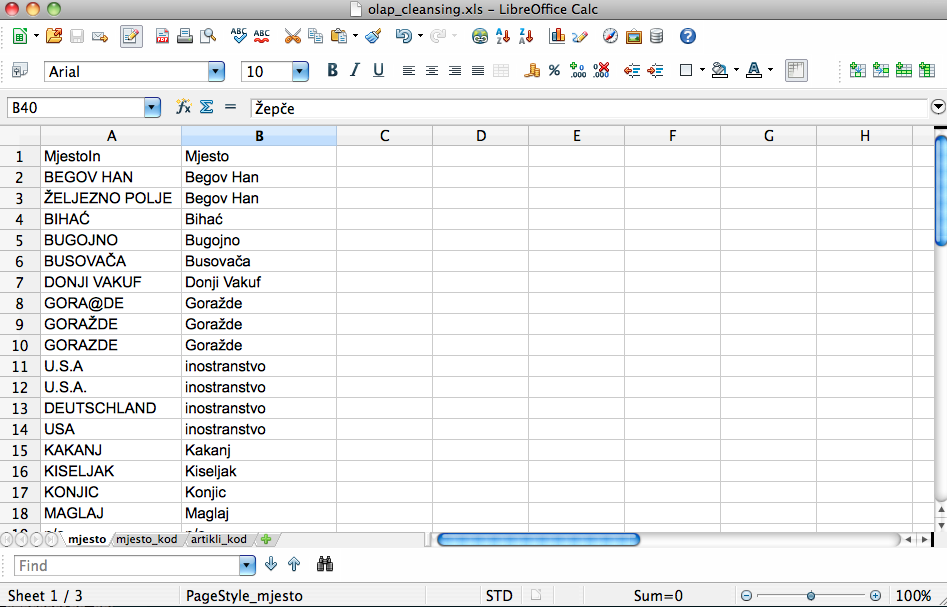
\includegraphics[width=15cm]{img/clean_mjesto.png}
\caption{`cleansing' F18 podataka -  klijenti - mjesta/gradovi}
\end{figure}


\begin{figure}[H]
\centering
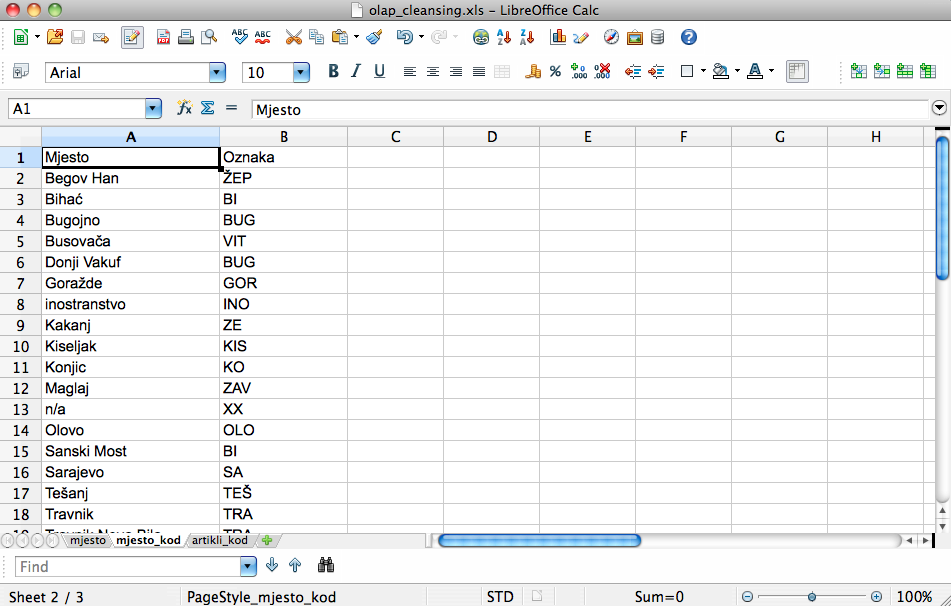
\includegraphics[width=15cm]{img/clean_mjesto_region.png}
\caption{F18 kodiranje regiona - klasifikacija mjesta/gradova}
\end{figure}


\begin{figure}[H]
\centering
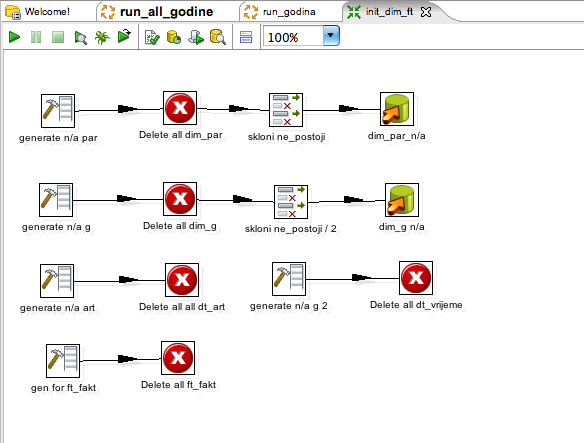
\includegraphics[width=15cm]{img/kettle_tr_init_dim_fpt.png}
\caption{Inicijalizacija `dimension' i `facts' tabela}
\end{figure}


\begin{figure}[H]
\centering
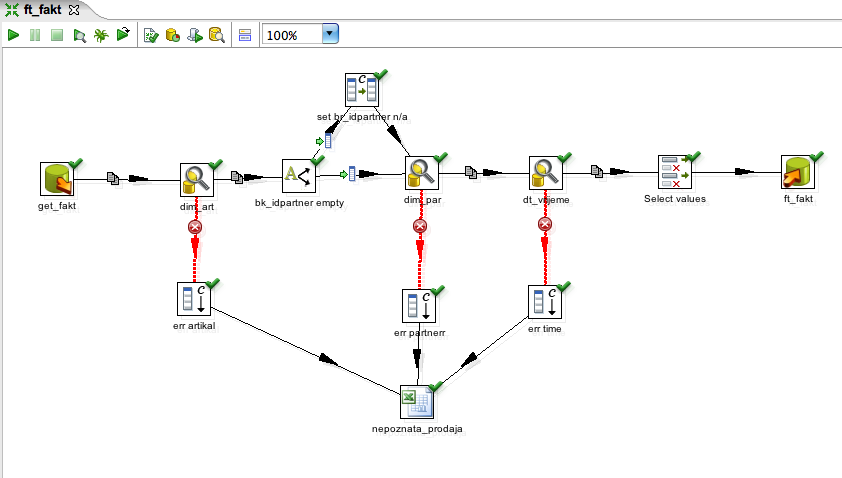
\includegraphics[width=15cm]{img/kettle_tr_ft_fakt.png}
\caption{Generacija "ft\_fakt" `facts' tabele za određenu poslovnu godinu}
\end{figure}


\begin{figure}[H]
\centering
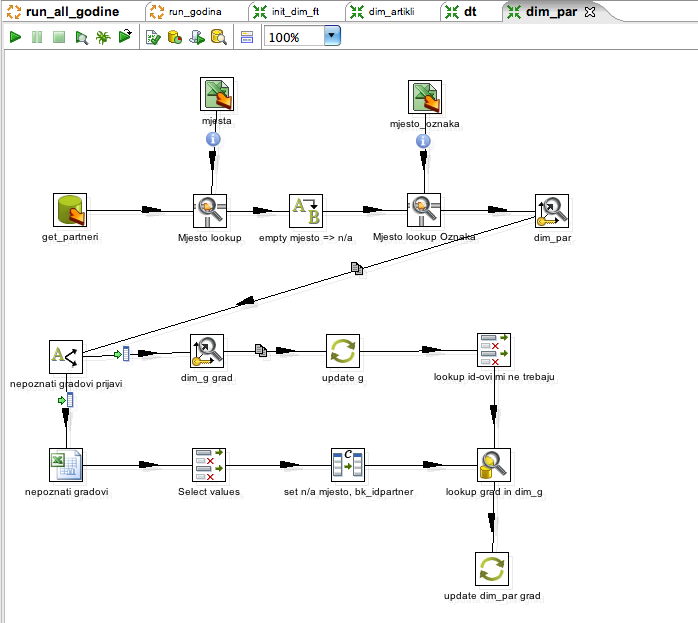
\includegraphics[width=15cm]{img/kettle_tr_dim_par.png}
\caption{Kettle transformacija: Generacija "dim\_par" i "dim\_g" `dimension' tabela za određenu poslovnu godinu}
\end{figure}

\begin{figure}[H]
\centering
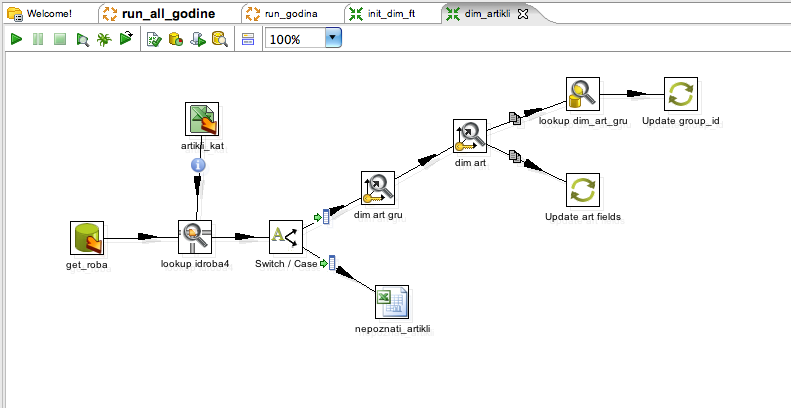
\includegraphics[width=15cm]{img/kettle_tr_dim_artikli.png}
\caption{Kettle transformacija: Generacija "dim\_art" i "dim\_art\_gru" `dimension' tabela za određenu poslovnu godinu}
\end{figure}


\begin{figure}[H]
\centering
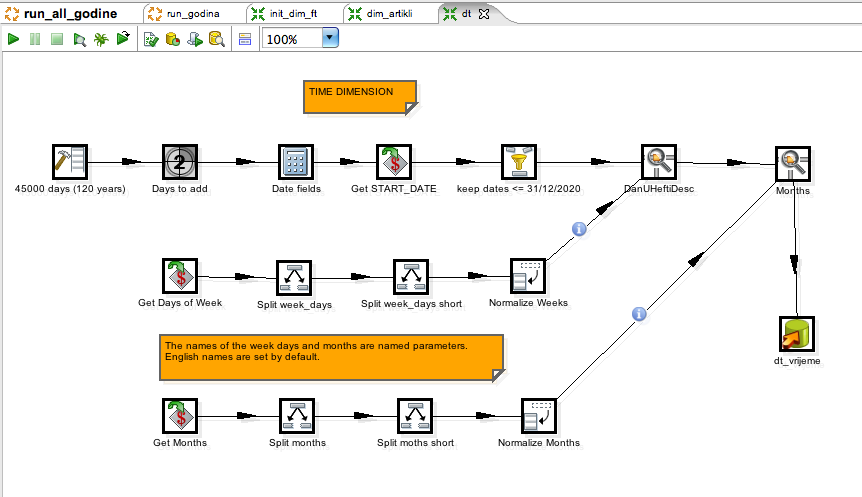
\includegraphics[width=15cm]{img/kettle_tr_dt.png}
\caption{Kettle transformacija: Generacija "dim\_dt" `dimension' tabele - vremenska dimenzija}
\end{figure}


\begin{figure}[H]
\centering
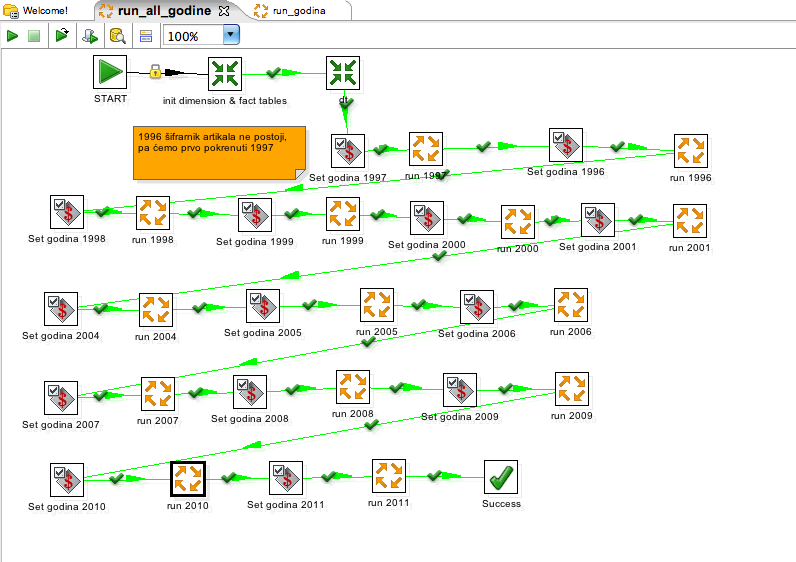
\includegraphics[width=15cm]{img/kettle_job_run_all.png}
\caption{Kettle job: inicijalizacija OLAP tabela, te generacija OLAP pdoataka za sve poslovne godine 1996-2011}
\end{figure}

\begin{figure}[H]
\centering
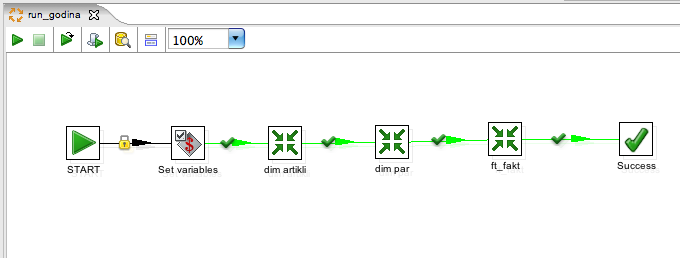
\includegraphics[width=15cm]{img/kettle_job_run_godina.png}
\caption{Kettle job: Generacija OLAP podataka iz F18 ERP izvora za jednu poslovnu godinu}
\end{figure}


\begin{figure}[H]
\centering
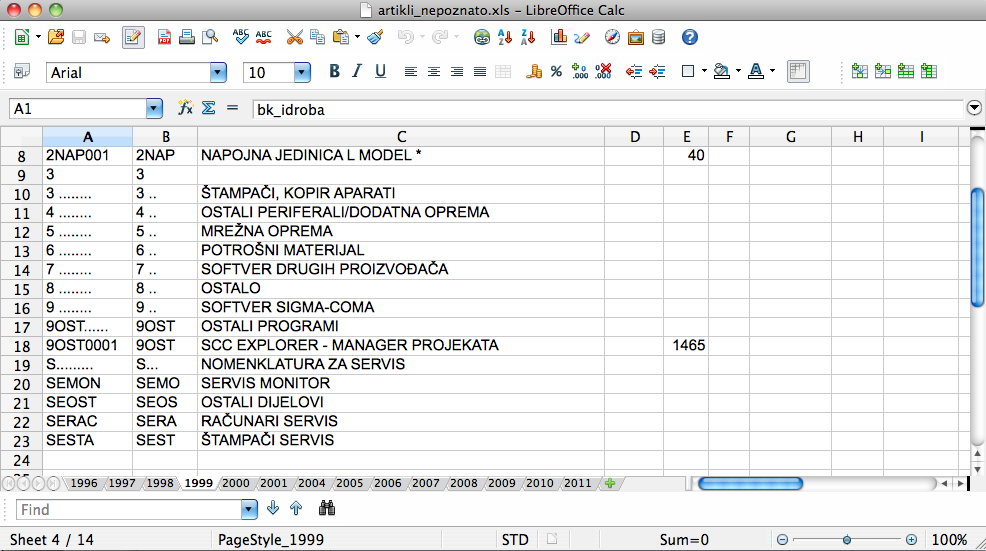
\includegraphics[width=15cm]{img/nepoznato_artikli.png}
\caption{Error reporting putem `spreadsheet' dokumenata - artikli za koje nisu definisani kodovi u olap\_cleansing tabelama}
\end{figure}

\begin{figure}[H]
\centering
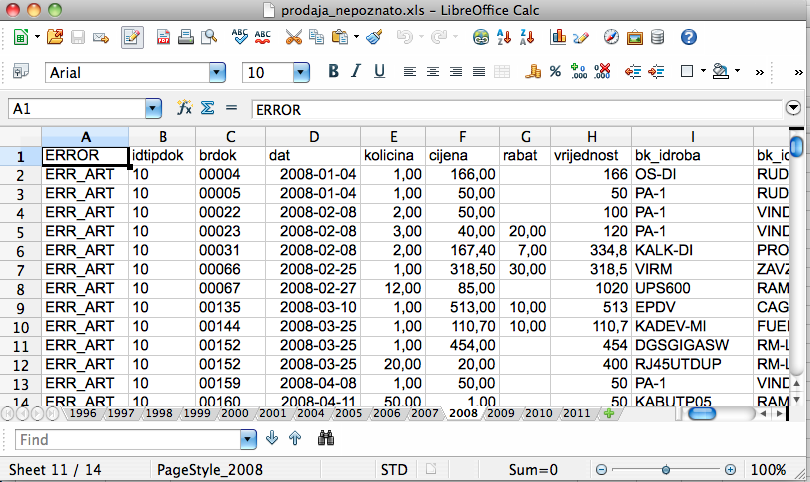
\includegraphics[width=15cm]{img/nepoznato_prodaja.png}
\caption{Dokumenti prodaje u kojima su neispravni podaci potrebni za popunjavanje dimension tabela (datum, klijent, roba) }
\end{figure}

\chapter{Iza case study-ja ?}

\section{Ne znam}

\subsection{dimension table}

\begin{figure}[h]
\centering
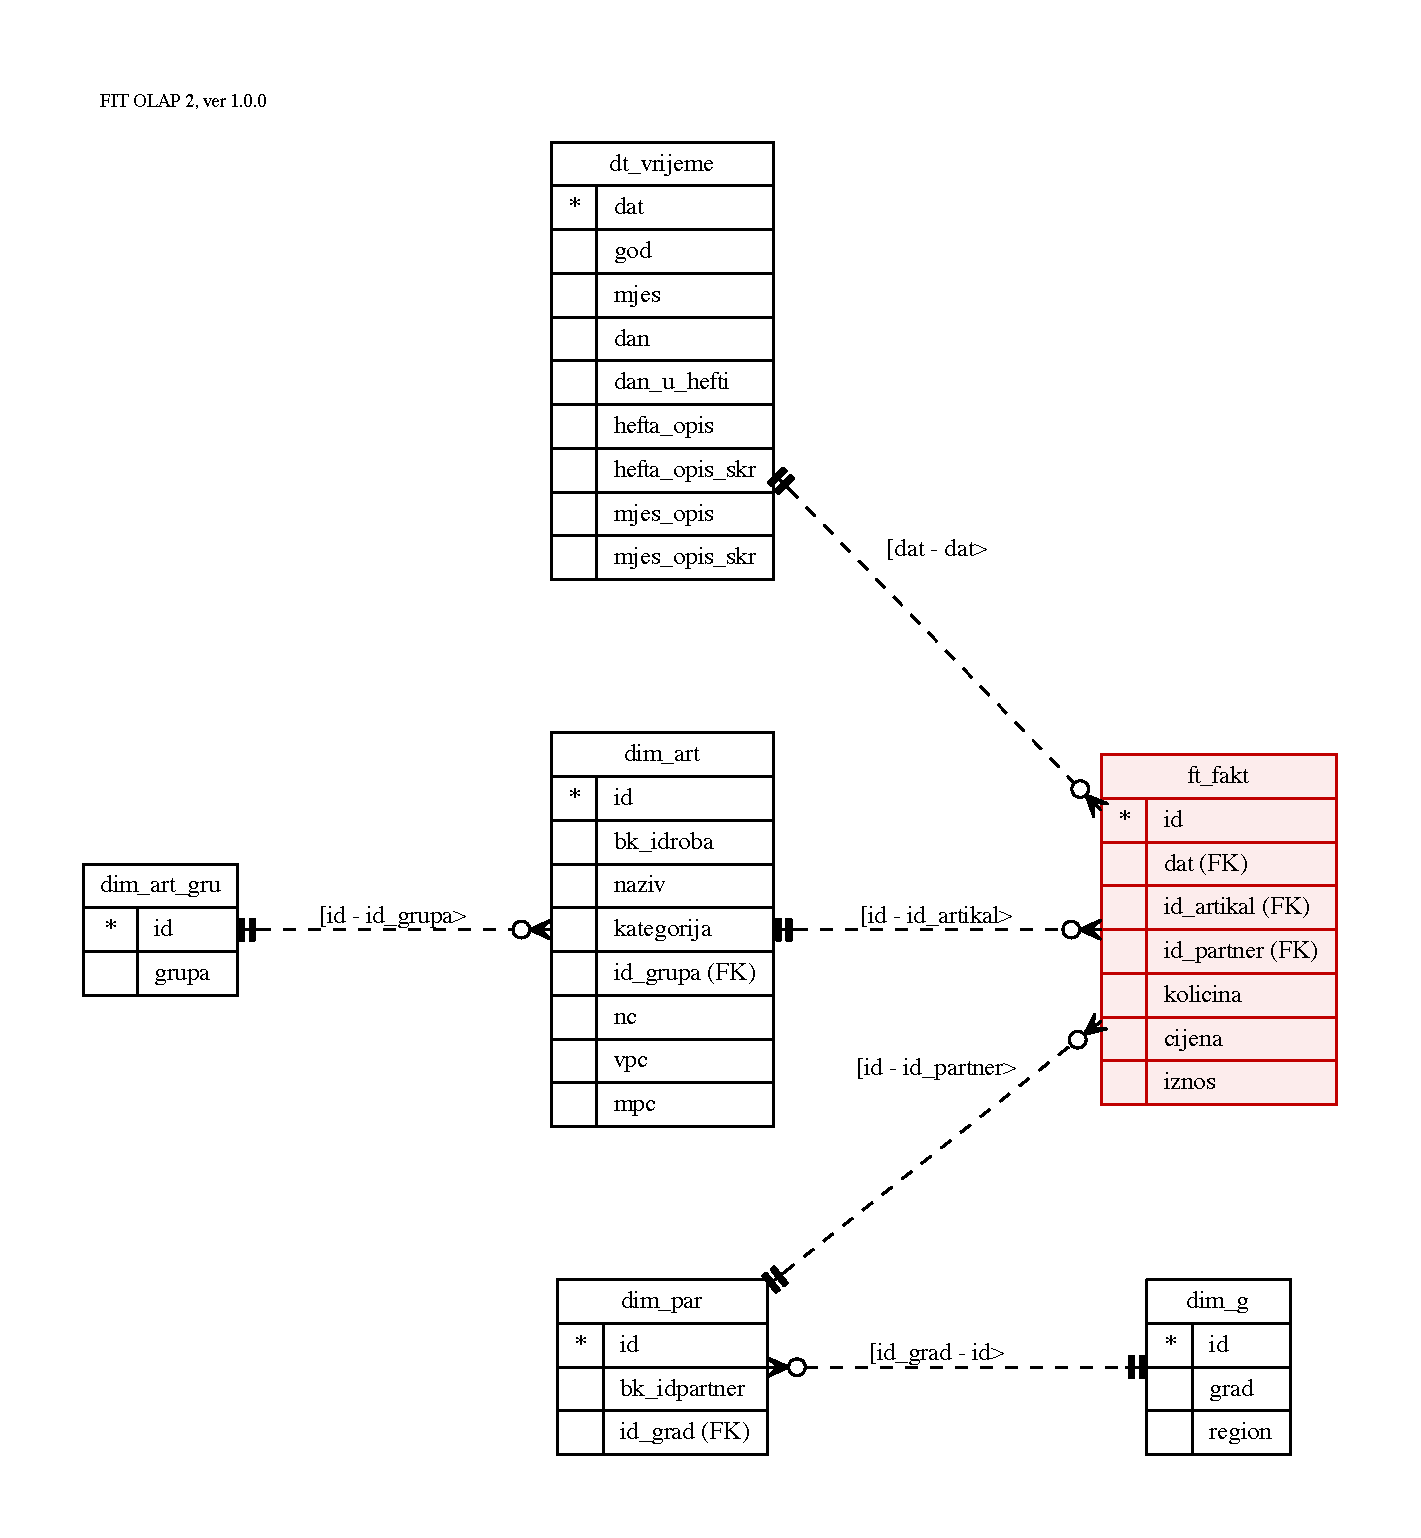
\includegraphics[width=15cm]{img/F18_olap.pdf}
\caption{OLAP schema}
\end{figure}



\subsection{facts table}



\subsection{ETL (Extract Transforn Load)}



\section{Analiza podataka}

\lstset{ %
   language=SQL,
   basicstyle=\small,
   numbers=left,
   numbersep=5pt,
   breaklines=true,
   backgroundcolor=\color{yellow!15},
   tabsize=2,
   keywordstyle=\color{blue},
   captionpos=b, 
   frame=none
}


\begin{figure}[H]
\centering
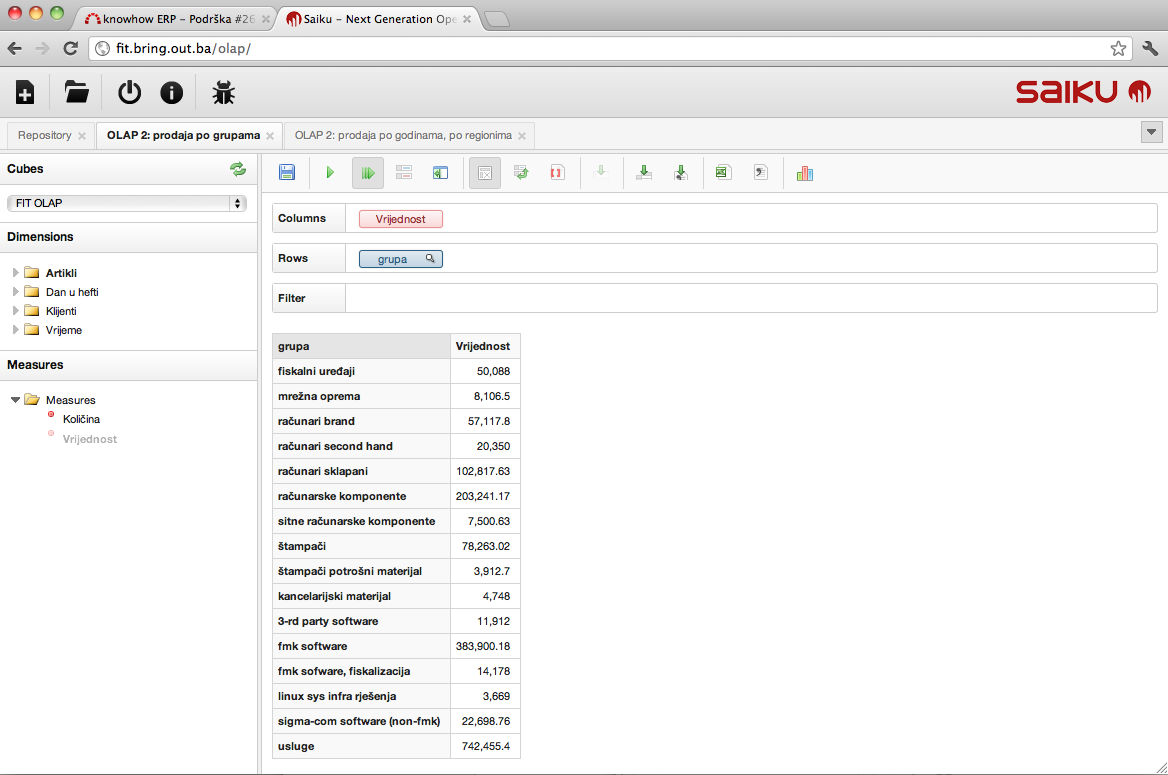
\includegraphics[width=15cm]{img/saiku_rpt_grupe}
\caption{Pregled prodaje po grupama artikala}
\end{figure}

\lstset{caption={Pregled prodaje po grupama artikala}}
\begin{lstlisting}
SELECT
NON EMPTY {Hierarchize({[Measures].[Vrijednost]})} 
ON COLUMNS,
  NON EMPTY {Hierarchize({[Artikli.artikli].[grupa].Members})} 
ON ROWS
FROM [FIT OLAP]
WHERE {Hierarchize({[Vrijeme.vrijeme].[All Vrijeme.vrijemes]})}
\end{lstlisting}


\begin{figure}[H]
\centering
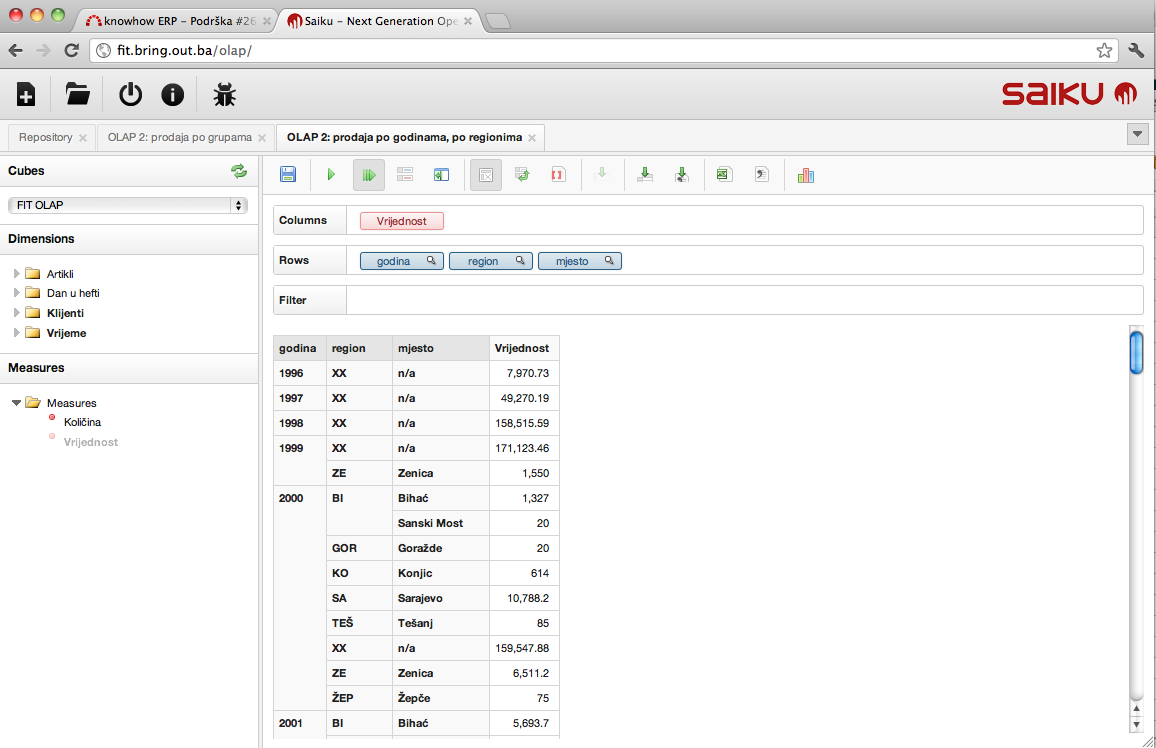
\includegraphics[width=15cm]{img/saiku_rpt_region}
\caption{Pregled prodaje po regionima, po godinama}
\end{figure}

\lstset{caption={Pregled prodaje po regionima}}
\begin{lstlisting}
SELECT
  NON EMPTY {Hierarchize({[Measures].[Vrijednost]})} 
ON COLUMNS,
  NON EMPTY 
    Hierarchize(
      Union(CrossJoin([Vrijeme.vrijeme].[godina].Members, 
      [Klijenti.klijenti].[region].Members), CrossJoin([Vrijeme.vrijeme].[godina].Members, 
      [Klijenti.klijenti].[mjesto].Members))
    ) 
ON ROWS
FROM [FIT OLAP]
\end{lstlisting}


\chapter{Zaključak}

\subsection{Ekspert}
Poznavanje sadržaja i postojećih struktura podataka.




\bibliography{literatura}
\bibliographystyle{fit}

\appendix

\chapter{Izvorni kod, dostupni resursi}
\label{chap:izvorni_kod}

\begin{enumerate}[labelindent=\parindent,leftmargin=*]
   \item OLAP mondrian, kettle transformacije i job-ovi, erviz modeli: \url{https://github.com/hernad/hello_bi}
   \item Latex kod ovog dokumenta \url{https://github.com/hernad/MIS/tree/master/latex}
   \item olap\_cleansing `spreadsheet' dokument \url{https://github.com/hernad/hello_bi/raw/master/olap_cleansing.xls}
   \item Saiku demo server online: \url{http://fit.bring.out.ba/olap/#}
\end{enumerate}

\chapter{Bilješke}

\begin{enumerate}
  \item Prva verzija ovog seminarskog rada, neuspješno \url{https://github.com/hernad/MIS/raw/master/knowhowERP_OLAP_blog_style.pdf}
  \item FIT OLAP 2 cube: \url{http://redmine.bring.out.ba/issues/26711}
\end{enumerate}

\end{document}
